\documentclass[11pt,a4 paper]{article}
\usepackage{subfiles}

\usepackage{amsmath, amsthm}
\usepackage[english]{babel}
\usepackage[T1]{fontenc}
\usepackage[utf8]{inputenc}
\usepackage[margin=2cm]{geometry}
\usepackage{graphicx}
%\usepackage{subfig}
\usepackage{caption}
\usepackage{siunitx}
\captionsetup{tableposition=top,font=small,width=0.8\textwidth}
\usepackage{booktabs}
\usepackage[table]{xcolor}
\usepackage[arrowdel]{physics}
\usepackage{mathtools}
\usepackage{tablefootnote}
\usepackage{amssymb}
\usepackage{enumitem}
\usepackage{subfigure}
\usepackage{multicol}
\setlist[description]{font={\scshape}} %style=unboxed,style=nextline
\usepackage{wrapfig}
\usepackage{float}
\usepackage{import}
\usepackage{floatflt}
\usepackage{url}
\usepackage{commath}
\usepackage{bm}
\usepackage[version=4]{mhchem}
\usepackage{nicefrac}
\usepackage{ifthen}
\usepackage{comment}
\usepackage[colorinlistoftodos,textsize=tiny]{todonotes}
\usepackage{hyperref}

\renewcommand*{\thefootnote}{\fnsymbol{footnote}}
\sisetup{exponent-product = \cdot}
\newcommand{\tc}{\,\mbox{tc}\,}
\newcommand{\Epsilon}{\mathcal{E}}
\newcommand{\half}{\frac{1}{2}}
\newcommand{\overbar}[1]{\mkern 1.5mu\overline{\mkern-1.5mu#1\mkern-1.5mu}\mkern 1.5mu}
\let\oldfrac\frac
\renewcommand{\frac}[3][d]{\ifthenelse{\equal{#1}{d}}{\oldfrac{#2}{#3}}{\nicefrac{#2}{#3}}}

\title{Timing}
\author{Andrea Grossutti, mat. 1237344\\Alessandro Lovo, mat. 1236048\\Leonardo Zampieri, mat. 1237351}
\date{\today}

\begin{document}

\maketitle

\section{Aims}
\begin{itemize}[noitemsep]
    \item Energy calibration of the organic scintillators and calculation of the energy resolution from the analysis of the Compton edge;
    \item Optimization of the external delay of the analogue CFTD to obtain the best time resolution;
    \item Study of the time resolution behaviour as a function of the energy;
    \item Comparison between the timing resolutions obtained from analogue and digital treatment of the signals;
    \item Measurement of the speed of light.
\end{itemize}

\section{Experimental setup}
The experimental setup consist of two collinear organic scintillators (DET 1 and DET 2), mounted on a sledge and facing each other. Between them there is a \ce{^22Na} source collimated by two lead bricks. The energy peaks of photons emitted by this source are shown in tab \ref{tab:gammavalue}.

Data are collected from the detectors through a electronic chain: a fan-in-fan-out quad module replies the signal of each detector and produces four copies of it; then, through a Constant Fraction Time Discriminator (CFTD), a logic signal is produced. The CFTD trigger threshold has been set so that the noise is discarded, while the interesting signals produce an output. From the CFTD the logic signal run through a coincidence unit, used as a trigger. Besides, the logic signal of DET 1 runs into the \emph{start} of a Time to Amplitude Converter (TAC) module, while the one from DET 2 passes through a delay module and then runs into the \emph{stop} of the TAC. A digitizer, triggered by the coincidence unit, acquires the energy spectra of both detectors and the time spectrum of the TAC.

\begin{table}[H]
    \centering
    \begin{tabular}{cccccccc}
        \toprule
        photopeak [keV] & Compton Edge [keV] \\
        \midrule
        $511.0$ & $340.7$\\
        $1274.537$ & $1061.7$ \\
        \bottomrule\vspace{0.01cm}
    \end{tabular}
    \caption{Gamma radiation for \ce{^22Na} from NuDat, \url{https://www.nndc.bnl.gov/nudat2/decaysearchdirect.jsp?nuc=22NA\&unc=nds}}
    \label{tab:gammavalue}
\end{table}

\section{Apparatus calibration}

\subsection{Calibration of DET 1 and 2}
Disabling the coincidence unit in order to collect both peaks of the \ce{^22Na} source, a spectrum for each detector is acquired. Due to the chemical composition of the detector (low Z materials), photopeaks are negligible and only the Compton effect is detected.

The observed Compton Edge (CE) is a convolution of the real CE with a gaussian noise whose width is the energy resolution of the detector $\sigma_{res}$; this convolution results in a shift of the maximum of the CE towards lower energies, so, in order to calibrate the detecters, we need to obtain an estimate of this shift.
By simulating\footnote{We used the formulas from N. Kudomi \emph{Energy calibration of plastic scintillators for low energy electrons by using Compton scattering of $\gamma$ rays}, Nuc. Instr. and Meth., 430 (1999), \url{www.elsevier.nl/locate/nima}} the effects on CE varying $\sigma_{res}$ (fig \ref{fig:sim:spectra}) we can compute the position of the peak $c_{sim}$ and its right hand side Half Width Half Maximum $w_{sim}$\footnote{We used this approach instead of a gaussian fit of the peaks because both in the simulation and in the experimental spectra the result of the fit was highly dependent on the range chosen for the fit, which is arbitrary. See also Dietze, Klein: \emph{Gamma-calibration of NE 213 scintillation counters}, Nuc. Instr. and Meth., 193 (1982), \url{https://doi.org/10.1016/0029-554X(82)90249-X}},
and  then correlate the simulated resolution $r_{sim} = \frac{w_{sim}}{c_{sim}}$ with $c_{sim}$ (fig \ref{fig:sim}).

We can now compute $c_{ch}$ and $w_{ch}$ for the experimental spectra in channels (fig \ref{fig:det12:calibr}, tab \ref{tab:calibr:fits}), noting that for the peak relative to the \SI{511}{\kilo\electronvolt} photon the half maximum needs to be computed with respect to the baseline due to the low energy Compton events of the \SI{1275}{\kilo\electronvolt} photon.\\
If we assume the calibration relation $E = a \cdot ch + b$, then the resolution in energy is:

\begin{equation*}
  r_E = \frac{w_E}{c_E} = \frac{a w_{ch}}{a c_{ch} + b} = \frac{w_{ch}}{c_{ch} + \frac[f]{b}{a}}
\end{equation*}

So we first assume $\frac[f]{b}{a} = 0$ to compute $r_E$, and then by imposing $r_E = r_{sim}$ we can find the peak positions in energy $c_E = c_{sim}(r_{sim})$ allowing us to compute $a$ and $b$ via linear fit. We can now update the value of $r_E$ and repeat the process. After a few iterations the process converges and gives us the results in tab \ref{tab:calibr:coeffs}.\\
This way we obtained also an estimate of the resolution of the detectors.

\begin{gather*}
  \sigma_{res}^{(1)} \sim 38\, \text{keV} \qquad
  \sigma_{res}^{(2)} \sim 35\, \text{keV}
\end{gather*}


\begin{figure}
  \centering
  \resizebox{0.8\textwidth}{!}{\import{img/}{sim_Compton_spectra.pgf}}
  \caption{Simulated Compton spectra with different values of $\sigma_{res}$ ($\sigma_{res} = 0$ is the real spectrum). Even if here the two peaks are represented together, they were analized independently.}
  \label{fig:sim:spectra}
\end{figure}

\begin{figure}
    \centering
    \resizebox{0.8\textwidth}{!}{\import{img/}{shift_from_CE.pgf}}
    \caption{Relation between the resolution of the peak and the peak position}
    \label{fig:sim}
\end{figure}

\begin{figure}
    \centering
    \resizebox{0.8\textwidth}{!}{\import{img/}{det12_calibrated.tex}}
    \caption{Position of CE's centroids and widths}
    \label{fig:det12:calibr}
\end{figure}

\begin{table}
  \centering
  \begin{tabular}{cccccccc}
    \toprule
    Det & $p$ [keV] & $c_{ch}$ & $w_{ch}$ & $c_E$ [keV] & $w_E$ [keV] & $r_E$ & $\sigma_{res}$ [keV]\\
    \midrule
    \#1 & 511 & $3440 \pm 9$ & $736 \pm 13$ & $290.2 \pm 0.7$ & $66 \pm 1$ & $0.227 \pm 0.004$ & $38.8 \pm 0.5$ \\
        & 1275 & $11312 \pm 9$ & $960 \pm 13$ & $994.1 \pm 0.8$ & $225 \pm 4$ & $0.086 \pm 0.001$ & $37.0 \pm 0.5$ \\
    \#2 & 511 & $4400 \pm 9$ & $768 \pm 13$ & $293.8 \pm 0.7$ & $60 \pm 1$ & $0.205 \pm 0.004$ & $35.7 \pm 0.6$ \\
        & 1275 & $13392 \pm 9$ & $960 \pm 13$ & $1000.5 \pm 0.7$ & $206 \pm 4$ & $0.075 \pm 0.001$ & $33.9 \pm 0.5$ \\
    \bottomrule
  \end{tabular}
  \caption{Centroids and widths of the CE peaks: $p$ is the photopeak energy. The errors for the values in channels come from a uniform distribution on the bin width of the histogram. The values of $c_E$, $w_E$, $r_E$ and $\sigma_{res}$ here are the ones after the calibration process converged.}
  \label{tab:calibr:fits}
\end{table}

\begin{table}
  \centering
  \begin{tabular}{cccccccc}
    \toprule
    Det & $a$ [keV] & $b$ [keV] \\
    \midrule
    \#1 & $0.0894 \pm 0.0002$ & $-17 \pm 2$ \\
    \#2 & $0.0786 \pm 0.0002$ & $-52 \pm 2$ \\
    \bottomrule
  \end{tabular}
  \caption{Calibrations coefficients after the calibration process converged}
  \label{tab:calibr:coeffs}
\end{table}

\subsection{Calibration of the TAC}

By changing the delay of the delay module just before the TAC's \emph{stop}, we can acquire different TAC peaks and use them for calibration (fig \ref{fig:tac:calibr}).
For each peak the centroid is found through gaussian fit on a small range around the maximum (tab \ref{tab:tac:calibr}).
%\todo[inline]{How have the centroid been found? -> A OCCHIO (mi spiace ma è la cruda realtà, non c'erano tanti altri modi visto che non erano fittabili in nessun modo (per quanto ne so io)). Anche le varianze sono a occhio ovviamente. Giuro che non mi metterò mai a costruire ponti.}

\begin{figure}
    \centering
    \resizebox{0.8\textwidth}{!}{\import{img/}{TACcalibr.tex}}
    \caption{Different peaks with different delays. Different height of the peaks are due to different acquisition time.}
    \label{fig:tac:calibr}
\end{figure}

\begin{table}
    \centering
    \begin{tabular}{cccccccc}
        \toprule
        Delay [ns] & Centroid [channel] \\
        \midrule
        $13$ & $2235\pm 20$ \\
        $17$ & $4950\pm 30$ \\
        $21$ & $7555\pm 30$ \\
        $25$ & $10390\pm 30$ \\
        $29$ & $13080\pm 40$ \\
        \bottomrule
    \end{tabular}
    \caption{TAC centroids.}
    \label{tab:tac:calibr}
\end{table}

The centroids are fitted using a linear relation:
\begin{gather*}
    t = m\cdot ch + q \\
    m = (1.477 \pm 0.005) \si{\pico\second} \qquad
    \chi^2/\text{ndf} = 11/3
\end{gather*}
% q = (9.71 +- 0.03)
where the $q$ value isn't reported, having no meaning. In fact, delays are introduced in a more complex system, which already have an internal delay: zero external delay therefore doesn't mean zero time in TAC.



\section{LEMO calibration}
A set of LEMO cables is provided. Setting external delay to $13\si{\nano\second}$ and inserting one by one each LEMO cable in series with the external delay module, 5-minutes datasets are acquired; computing the difference between the observed centroids and the centroid without LEMO cable previously measured, and converting it with the calibration parameter, the time-length of each LEMO cable is computed.

\begin{figure}[H]
    \centering
    \resizebox{0.8\textwidth}{!}{\import{img/}{lemo.tex}}
    \caption{Some of the peaks of the LEMO cables}
    \label{fig:lemo}
\end{figure}

\begin{table}[H]
    \centering
    \begin{tabular}{cccccccc}
        \toprule
        LEMO ID & LEMO length [cm], $\pm 0.1$ & LEMO time [ns]\\
        \midrule
        $6$ & $22.5$ & $1.17\pm0.04$\\
        $7$ & $23.0$ & $1.15\pm0.04$\\
        $2$ & $53.5$ & $2.70\pm0.03$\\
        $13$ & $53.5$ & $2.71\pm0.05$\\
        $4$ & $101.0$ & $5.12\pm0.04$\\
        $5$ & $101.0$ & $5.08\pm0.07$\\
        \bottomrule
    \end{tabular}
    \caption{LEMO cables}
    \label{tab:lemo}
\end{table}

\begin{figure}[H]
    \centering
    \resizebox{0.8\textwidth}{!}{\import{img/}{lemo_length.tex}}
    \caption{Relation between LEMO length and time: as expected, the dependence is confirmed.}
    \label{fig:lemo_length}
\end{figure}
\todo[inline]{Serve davvero fig \ref{fig:lemo_length}? Sarebbe piuttosto meglio mettere il grafico del fit lineare della calibrazione dei 5 picchi TAC}



\section{CFTD delay optimization}

The CFTD superimposes a delayed copy of the signal to an inverted reduced one. This delay must be properly set using LEMO cables to optimize the TAC resolution. With only the default delay, the signal detected by the TAC is large and not gaussian (see fig. \ref{fig:delay:bad}); after some tests, a setup which lead to a better resolution and a more gaussian-like output is obtained.

\begin{figure}
    \centering
    \resizebox{0.8\textwidth}{!}{\import{img/}{delay_optim_bad.tex}}
    \caption{Initial situation: large not-guassian shape.}
    \label{fig:delay:bad}
\end{figure}

Different combination of LEMO cable have been inserted in series with the pre-set delay; every time the configuration changed, the WALK ADJ potentiometer has been regulated to minimize the dispersion (see fig. \ref{fig:oscilloscope}) at the zero-crossing point of the signals.

\begin{figure}
    \centering
    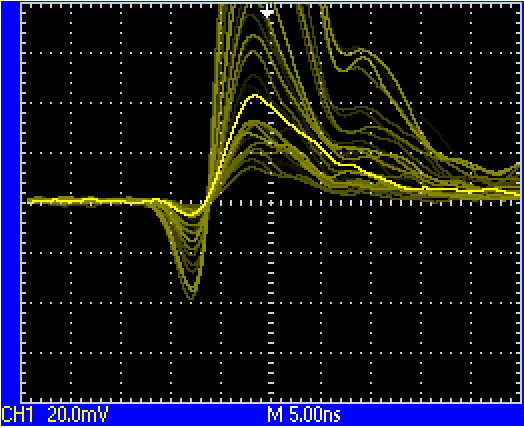
\includegraphics[width=0.7\textwidth]{img/oscilloscope.jpg}
    \caption{Monitor CFTD signal triggered on CFTD output, seen by the oscilloscope.}
    \label{fig:oscilloscope}
\end{figure}

Fitting the obtained peaks with a gaussian and relating them to the delay inserted in the CFTDs (after some tests, we noticed that the optimal setup is with the same delay in both CFTDs), we obtain the result in fig \ref{fig:CFTD:delay}. As can be seen from the figure, a minimum is found at about $3\si{\nano\second}$ of delay (LEMO 13 for DET 1 and LEMO 2 for DET 2). Considering the pre-set delay (around $2\si{\nano\second}$), this lead to a optimal delay of around $5\si{\nano\second}$, that is about $80\%$ the rise time of the detector signal ($\sim6\si{\nano\second}$) as expected.

\begin{figure}[H]
    \centering
    \resizebox{0.8\textwidth}{!}{\import{img/}{CFTDdelay.tex}}
    \caption{Optimization of the CFTD delay.}
    \label{fig:CFTD:delay}
\end{figure}

The minimum configuration has been kept for all the following measurements.



\section{Time resolution in function of energy range}
In order to have a wider Compton energy spectra, we acquired 20 hours of data using a \ce{^60Co} source. This source decays emitting two photons of energy around 1\si{\mega\electronvolt}: a few of them are emitted back-to-back and hence can trigger the coincidence unit (fig \ref{fig:Co:spectra}).\\
We can now proceed by filtering in energy the spectra and looking how the resolution of the TAC peak behaves. Since the TAC peak has a fat-tailed distribution, the gaussian fit is not accurate, so we used the Full Width Half Maximum (FWHM) as a quantifier of the resoultion of the peaks.
The filtering can be done either by setting a Lower Energy Threshold (LET) or by selecting a window in energy, i.e. keeping only the data with energy between the LET and an Upper Energy Threshold (UET). The results are shown in fig \ref{fig:Co:results}.

\begin{figure}
    \centering
    \resizebox{0.8\textwidth}{!}{\import{img/}{Co_spectra.tex}}
    \caption{Energy spectra of the two detectors with \ce{^60Co} source.}
    \label{fig:Co:spectra}
\end{figure}

\begin{figure}
    \centering
    \resizebox{0.8\textwidth}{!}{\import{img/}{Co.tex}}
    \caption{When computing the FWHM, the peaks had been properly rebinned in order to have them sufficiently smooth. The errors on the FWHMs come from a uniform distribution on the bin width.}
    \label{fig:Co:results}
\end{figure}

From fig \ref{fig:Co:results} we can see that the resolution improves dramatically as we discard the events at lower energy, and then remains almost constant as the LET increases. Considering that using only a LET implies that as it increases the number of discarded data increases too, the best choice for the LET is at around \SI{200}{\kilo\electronvolt}. On the other hand when using both a LET and a UET, given the shape of the \ce{^60Co} spectrum, moving the energy window does not drastically affect the number of discarded events. So in this case the best choice is a window near the Compton Edge.



\section{Speed of light}
The detectors have been placed such that they're about $1.70\si{\metre}$ away. The \ce{^22Na} source has been placed firstly near DET 1 and then near DET 2, and the TAC signal has been acquired (one hour for each configuration); then, the centroids $\mu_1$ and $\mu_2$ of the two measurements have been found through a gaussian interpolation. Measuring the distance between the two source positions $d$, the light speed can be computed.

Observe that the two centroids have been firstly subtracted keeping them in channel and then calibrated, to prevent the introduction of correlation between the two measures.

The errors have been propagated as statistical errors. Note the high error on the distance between the positions of the source, due to the width of the source.

\begin{gather*}
    \mu_1 = (16433 \pm 2)\si{channel}\\
    \mu_2 = (8966 \pm 2)\si{channel} \\
    d = (161.9 \pm 0.5) \si{\centi\metre} \\
    c = \frac{2d}{(\mu_1-\mu_2)m} = (2.94 \pm 0.01 )\cdot 10^8 \si{\metre\per\second}
\end{gather*}

\todo[inline]{Dire qualcosa sul fatto ch siamo incompatibili con il valore teorico}

\section{A-Posteriori CFTD}
During the last day, we disabled the digitizer's FPGA and acquired two datasets of raw waveforms directly from the detectors. This allows us to simulate an a-posteriori software CFTD, and compare it with the analogic one.

\subsection{Waveforms}
\begin{figure}[H]
    \centering
    \begin{subfigure}[Analogic CFTD]{
        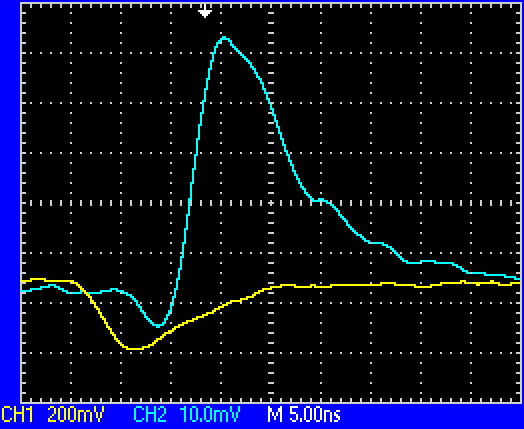
\includegraphics[width=0.38\textwidth]{img/waveform_osc.jpg}
        \label{fig:waveform_osc}
    }\end{subfigure}
    \begin{subfigure}[APosteriori CFTD]{
        \resizebox{0.58\textwidth}{!}{\import{img/}{waveform_sim.tex}}
        \label{fig:waveform_sim}
    }\end{subfigure}
    \caption{Waveforms (yellow) and monitor signals (cyan) for analogic and software CFTD, set with the same parameters (fraction = $20\%$, delay = $\sim 5\si{\nano\second}$)}
    \label{fig:waveform}
\end{figure}

As can be seen from fig. \ref{fig:waveform}, the shape of waveform and signal is similar for the two system. Rise time (about $6\si{\nano\second}$) and falling time (about $20\si{\nano\second}$) are the same. The signal, however, is very short in time and the low time resolution of the digitizer (a sample each $1$ns) result in a rougher waveform.


\subsection{Energy spectra}
\begin{figure}[H]
    \centering
    \resizebox{0.7\textwidth}{!}{\import{img/}{aposteriori_energy.tex}}
    \caption{APosteriori energy spectra.}
    \label{fig:aposteriori_energy}
\end{figure}

\todo[inline]{Si potrebbe sovrapporre lo spettro analogico (eventualmente normalizzando i due istogrammi)}

Integrating the waveform (substracted of the baseline) over the domain, an energy spectra can be computed. As can be seen comparing fig. \ref{fig:aposteriori_energy} with fig. \ref{fig:det12:calibr}, here only the $511\si{\kilo\electronvolt}$ peak is visible: the trigger set on coincidences and the low acceptance of the digitized cut away the higher peak.

Even with only one peaks, the comparison with the previous calibration permit us to make a rough calibration using position of peak and half maximum (in red in figure).

Note that in this plot there are some energy that are below zero; this is due to the combination between the low trigger threshold and the detectors resolution, the convolution of which result in a tail in negative energies.

\subsection{CFTD parameters}
\todo[inline]{Ma tipo, se quando calcoliamo il crossing point invece di interpolare i valori con segmenti usiamo una curva più morbida, come cambiano i risultati? Se la cosa implica troppo tempo ignoratemi (:}
For each dataset, the following procedure is followed:
\begin{itemize}[noitemsep]
    \item Coincidences are searched, i.e. events that are recorded by both the detectors;
    \item For each event, a simulated CFTD is applied to the two waveforms and zero crossing are computed;
    \item For each event, the time difference between the zero crossings in the two detector is computed;
    \item The distribution of the time difference is builded: mean, sigma (defined as the square root of the normalized centered second moment of data) and kurtosis (a measure of the \emph{gaussianity} of the distribution, equals $0$ for a perfect gaussian) are computed;
\end{itemize}
\todo[inline]{And for awful gaussian the values of kurtosis are positive or negative?}
This procedure is repeated for different combination of CFTD delay (from $1$ to $10\si{\nano\second}$, with $0.25\si{\nano\second}$ step) and attenuation fraction (from $0.1$ to $0.9$, with $0.1$ step) and the plots of sigma and kurtosis are builded.
\todo[inline]{Io farei i due grafici seguenti usando lo stesso colore per valori belli (es. rosso) e lo stesso per valori brutti (es. blu). Può essere che sia già cosi e che io non abbia capito come funziona il Kurtosis e/o perché abbia valori negativi oggi (ieri eran positivi). Ma sono abbastanza sicuro di avere ragione e che quindi sia carino invertire i colori di uno dei due.}
\todo[inline]{Siamo sicuri che con un delay di ~9.5ns le due onde (invertita e attenuata) si sovrappongano ancora? Giusto per esser sicuri che i risultati abbiano senso. Domani comunque vedo di verificare, per ora lo scrivo così domani mi ricordo.}

\begin{figure}[H]
    \centering
    \resizebox{0.7\textwidth}{!}{\import{img/}{sigma_2D.tex}}
    \caption{Sigma of the time differences distribution as function of CFTD parameters.}
    \label{fig:sigma2D:sim}
\end{figure}

\todo[inline]{I valori nell'angolo in basso a sx del kurtosis han ben poco senso, li cancellerei piuttosto che lasciarli come valori più attendibili}

\begin{figure}[H]
    \centering
    \resizebox{0.7\textwidth}{!}{\import{img/}{kurt_2D.tex}}
    \caption{Kurtosis of the time differences distribution as function of CFTD parameters.}
    \label{fig:kurt:sim}
\end{figure}

Note that the low-delay low-fraction corner points has been discarded: their means result incompatible with the others and their sigma extremely high, reflecting errors (probably due to low digitizer time resolution) in zero-crossings finding.

The kurtosis values are very high: plotting one of the distribution, it's clear they aren't gaussian-like, but triangular-like, again because of digitizer resolution. It records only 5-6 points in the rising time, digitally sampled; the zero crossing is therefore individuated by interpolating two (or in very good conditions four) points: a very rough interpolation! Assuming the uniform probability density function (PdF) typical of digital instruments and convolving the start and stop PdF, they result in a triangular-like PdF as experimental results show.
\todo[inline]{In conclusions make some discussion about the fact that analogic CFTD is better than offline one for these reasons (despite the scazzo col cambiare i cavetti)}
\todo[inline]{Qui, una volta scelto il valore ottimale  di delay e attenuation fraction, potremmo inserire un grafico in cui, per un solo canale alla volta, una volta allineati i picchi originali applichiamo il CFTD su tutti i campioni e poi li grafichiamo tutti in un TH2F di quelli belli colorati (capitemi, è quello che mi ha fatto fare il prof l'ultimo giorno di esperimento). Se siam stati bravi dovremmo vedere la maggior parte delle onde passare per il canale a cui abbiamo allineato i picchi inizialmente.}

\subsection{Time resolution and energy threshold}

\begin{figure}[H]
    \centering
    \resizebox{0.8\textwidth}{!}{\import{img/}{sigma_sim.tex}}
    \caption{Sigma as a function of energy threshold.}
    \label{fig:sigma:sim}
\end{figure}

\todo[inline]{Non sarebbe meglio mettere FWHM invece della $\sigma$ per confrontare meglio i due grafici (anche semplicemente facendo $FWHM = 2\sqrt{2\ln{2}} \sigma$)}

\todo[inline]{Volendo si potrebbe fare la stessa analisi di risoluzione del Co sul sodio e confrontare la versione analogica e quella digitale}

Finally, sigma has been computed varying the energy threshold, replying the procedure done for cobalt and setting the same CFTD parameters. As can be seen in figure comparing fig. \ref{fig:Co:results} with fig. \ref{fig:sigma:sim}, the $y$ axis scale is different: there are about 2 order of magnitude of difference. This lead us to impute the main contribute to the sigma to the sampling done by the digitizer. In the same figure, a strong growth in sigma can be seen in high $LET$ zone, probably due to the lack of data at high energy to make a precise mean. On the other hand, a minimum can be seen in the black line: This minimum is however not so relevant observing the $\sigma$ scale.




\end{document}
